%% ===================================================================
%% PART III
%% ===================================================================
\part{Rigidity, vector-space partitions and universality}

Throughout Part~III, $C$ is a \emph{minimal non-embedded box} of nullity $k$. We use the reduced code (Proposition~\ref{prop:series}): $p$ denotes the number of coordinates of the reduced code, which we identify with $C$, so blocks of partitions of $\one$ have sizes measured in the reduced code and $\sum_{B\in P}|B|=p$. All statements in this part are statements about the reduced code; by Proposition~\ref{prop:series} they transfer to blow-ups.

%% -------------------------------------------------------------------
\section{Circuit rigidity}\label{sec:rigidity}

\begin{theorem}[Rigidity; \gid{G10-R}]\label{thm:rigid}
Let $C$ be a minimal non-embedded box. Then:
\begin{enumerate}[label=(\alph*)]
\item every word $w\in C\setminus\{0,\one\}$ has a \emph{unique} decomposition into pairwise disjoint circuits;
\item the word $\one$ has $\beta=|\Part|\ge2$ decompositions;
\item the number of circuit families (nonempty sets of pairwise disjoint circuits) of $C$ is $2^k-2+\beta$, and a family whose union is not $[n]$ is determined by its union.
\end{enumerate}
\end{theorem}

\begin{proof}
(a)~If $w\ne0,\one$ had two decompositions $S\ne T$, the set $U=\supp w\ne[n]$ would have two partitions, contradicting Theorem~\ref{thm:F1}. (b)~is Theorem~\ref{thm:F1}. (c)~Families with union $\ne[n]$ correspond bijectively to words $w\in C\setminus\{0,\one\}$ (each such word has exactly one decomposition, by~(a), and each family determines its union word); there are $2^k-2$ such words. The families with union $[n]$ are the $\beta$ elements of $\Part$.
\end{proof}

\src{\gid{G10-R}, GEO-I v010 \texttt{MATHEMATICS.md} \S1.4 (\PROVED): rigidity and the count of families. The proof above is a direct consequence of Theorem~\ref{thm:F1}.}

The converse also holds and shows that rigidity is not just a consequence but a characterisation.

\begin{proposition}[Rigidity characterises minimality]\label{prop:rigid-char}
A code $C$ with $\one\in C$ is minimal non-embedded if and only if $\one$ has at least two decompositions into disjoint circuits and every $w\in C\setminus\{0,\one\}$ has exactly one.
\end{proposition}

\begin{proof}
($\Rightarrow$)~Theorem~\ref{thm:rigid}. ($\Leftarrow$)~$C$ is non-embedded by Theorem~\ref{thm:E1}. Let $i\in[n]$. A nonzero word of $C_{(i)}$ is a word $w\in C$ with $w_i=0$, so $w\ne\one$ and $w$ has a unique decomposition into circuits of $C$; these circuits lie in $\supp w$, so they avoid $i$ and are circuits of $C_{(i)}$ (Lemma~\ref{lem:shortcirc}). Hence no word of $C_{(i)}$ has two decompositions in $C_{(i)}$, and $C_{(i)}$ is embedded by Theorem~\ref{thm:E1}.
\end{proof}

\src{The converse is noted here; it was not found stated in the release files read.}

The bijection of words and circuit families in Theorem~\ref{thm:rigid} makes the combinatorics of a minimal box unusually rigid: the family structure is that of a \emph{linear space with exactly one failure of unique factorisation}, and the next section shows that this single failure is organised by a vector-space partition.

%% -------------------------------------------------------------------
\section{Vector-space partitions from partitions of the all-ones word}\label{sec:vsp}

Recall that $\Part$ is the set of partitions $P$ of $[n]$ (in the reduced code, of the $p$ coordinates) into circuits; $m_P=|P|\ge2$ is the number of blocks (Corollary~\ref{cor:minprops}), and each block has size $\ge2$. Put
\[
V_P=\spn P=\Bigl\{\bigoplus_{B\in J}B:\ J\subseteq P\Bigr\}\le C,\qquad\dim V_P=m_P,\qquad\{0,\one\}\subseteq V_P.
\]
(Lemma~\ref{lem:span}.)

\begin{lemma}[Existence]\label{lem:vsp-exist}
Every $w\in C\setminus\{0,\one\}$ lies in $V_P$ for at least one $P\in\Part$.
\end{lemma}

\begin{proof}
Both $w$ and $\one\oplus w$ are nonzero words of $C$ (neither equals $\one$ or $0$ because $w\ne0,\one$). Decompose each into disjoint circuits (Lemma~\ref{lem:circuit-basic}(b)); their supports are complementary, so the union of the two decompositions is a partition $P$ of $[n]$ into circuits, and $w$ is the sum of the blocks coming from the decomposition of $w$: $w\in V_P$.
\end{proof}

\begin{lemma}[Uniqueness]\label{lem:vsp-uniq}
If $w\in V_P\cap V_Q$ with $w\ne0,\one$ then $P=Q$.
\end{lemma}

\begin{proof}
Write $w=\bigsqcup_{B\in J}B$ with $J\subseteq P$ and $w=\bigsqcup_{B'\in J'}B'$ with $J'\subseteq Q$. Both are decompositions of $w$ into disjoint circuits, so by rigidity (Theorem~\ref{thm:rigid}(a)) $J=J'$ as sets of circuits. Likewise $\one\oplus w$ is the union of $P\setminus J$ and of $Q\setminus J'$, so $P\setminus J=Q\setminus J'$. Hence $P=J\cup(P\setminus J)=J'\cup(Q\setminus J')=Q$.
\end{proof}

\begin{theorem}[Vector-space partition; \gid{G11-L5}]\label{thm:vsp}
Let $C$ be a minimal non-embedded box of nullity $k$. The subspaces $V_P$ ($P\in\Part$) satisfy $V_P\cap V_Q=\{0,\one\}$ for $P\ne Q$ and $\bigcup_PV_P=C$. Consequently the subspaces
\[
\bar V_P=V_P/\langle\one\rangle\ \le\ C/\langle\one\rangle\cong\F_2^{k-1}
\]
of dimension $m_P-1\ge1$ form a \emph{vector-space partition} of $\F_2^{k-1}$: every nonzero vector lies in exactly one $\bar V_P$. A part has dimension $1$ if and only if $P$ has exactly two blocks.
\end{theorem}

\begin{proof}
For $w\ne0,\one$ Lemmas~\ref{lem:vsp-exist} and~\ref{lem:vsp-uniq} give exactly one $P$ with $w\in V_P$; also $0,\one\in V_P$ for all $P$, so $V_P\cap V_Q=\{0,\one\}$ and the union is $C$. Passing to $C/\langle\one\rangle$, the images of $V_P\setminus\{0,\one\}$ are pairwise disjoint and cover the nonzero classes; dimension is $m_P-1$.
\end{proof}

\src{\gid{G11-L5}, GEO-I v011 \texttt{MATHEMATICS.md} \S1.2--1.3 (\PROVED). The terminology follows the standard notion of a vector-space partition \cite{Heden2012}: a family of subspaces such that each nonzero vector lies in exactly one member (only the abstract page of the survey was read).}

\begin{remark}[Type]\label{rem:type}
The multiset $\{m_P-1: P\in\Part\}$ is the \emph{type} of the partition in the usual sense. For example the minimal reduced box with $k=4$, $p=6$ has four parts of dimension $1$ and one of dimension $2$ (four two-block partitions of $\one$ and one three-block partition); for $E_4$ the type is $[1^3]$ in $\F_2^2$; for $X=\AG(k-1,2)$ it is $[1^{2^{k-1}-1}]$, the trivial partition of $\F_2^{k-1}$ into its $2^{k-1}-1$ points.
\end{remark}

\begin{figure}[ht]
\centering
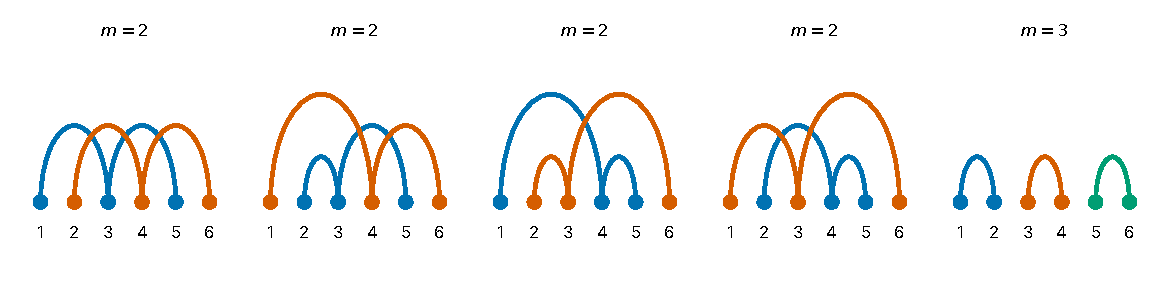
\includegraphics[width=0.95\textwidth]{figures/fig08_two_partitions.pdf}
\caption{The five partitions of the all-ones word of the minimal reduced box with $k=4$, $p=6$ (representative $X=\{8,\dots,13\}\subset\AG(3,2)$): four partitions into two circuits of size~$3$, one into three circuits of size~$2$. \figdesc{exact data from the circuit list; blocks drawn as arcs over the six coordinates.}}\label{fig:twopart}
\end{figure}

\begin{figure}[ht]
\centering
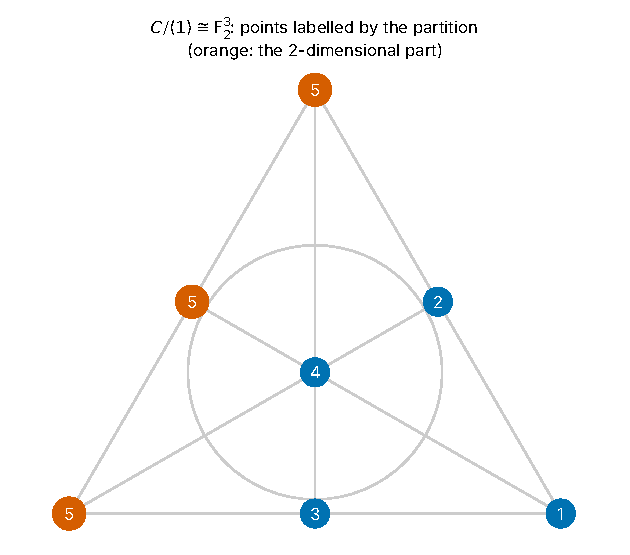
\includegraphics[width=0.8\textwidth]{figures/fig09_vsp_fano.pdf}
\caption{The vector-space partition of $C/\langle\one\rangle\cong\F_2^3$ (the Fano plane) for the same box: four singleton parts (points) and one part of dimension $2$ (a line). \figdesc{points are the seven nonzero cosets of $\langle\one\rangle$, computed exactly; drawing is schematic.}}\label{fig:fano}
\end{figure}

%% -------------------------------------------------------------------
\section{The counting identity}\label{sec:counting}

\begin{theorem}[Counting identity; \gid{G11-L5}]\label{thm:counting}
For a minimal non-embedded box of nullity $k$,
\[
\sum_{P\in\Part}\bigl(2^{m_P}-2\bigr)=2^k-2,\qquad\text{equivalently}\qquad\sum_{P\in\Part}\bigl(2^{m_P-1}-1\bigr)=2^{k-1}-1 .
\]
In terms of $n_m=\#\{P: m_P=m\}$: $\sum_{m\ge2}n_m(2^m-2)=2^k-2$.
\end{theorem}

\begin{proof}
Each $V_P\setminus\{0,\one\}$ has $2^{m_P}-2$ elements and these sets partition $C\setminus\{0,\one\}$ (Theorem~\ref{thm:vsp}), which has $2^k-2$ elements.
\end{proof}

\begin{corollary}\label{cor:counting-consequences}
(a)~$n_2\le2^{k-1}-1$, with equality iff all partitions of $\one$ have exactly two blocks. (b)~$\beta=|\Part|\le 2^{k-1}-1$. (c)~If $n_m=0$ for all $m\ge4$ then $2n_2+6n_3=2^k-2$.
\end{corollary}

\begin{proof}
Immediate from $2^m-2\ge2$ for $m\ge2$ and Theorem~\ref{thm:counting}.
\end{proof}

\begin{example}[Checks]\label{ex:counting}
$E_4$ ($k=3$): $3\cdot(4-2)=6=2^3-2$. The minimal reduced box with $k=4,p=6$: $4\cdot2+1\cdot6=14=2^4-2$. $\AG(3,2)$ ($k=4$, $p=8$): $7\cdot2=14$. The classes with $k=5$, $p=10$ and $n_2=12$, $n_3=1$: $12\cdot2+6=30=2^5-2$. All $231$ minimal reduced classes with $k\le6$ satisfy the identity (exact check; Appendix~\ref{app:repro}).
\end{example}

\begin{figure}[ht]
\centering
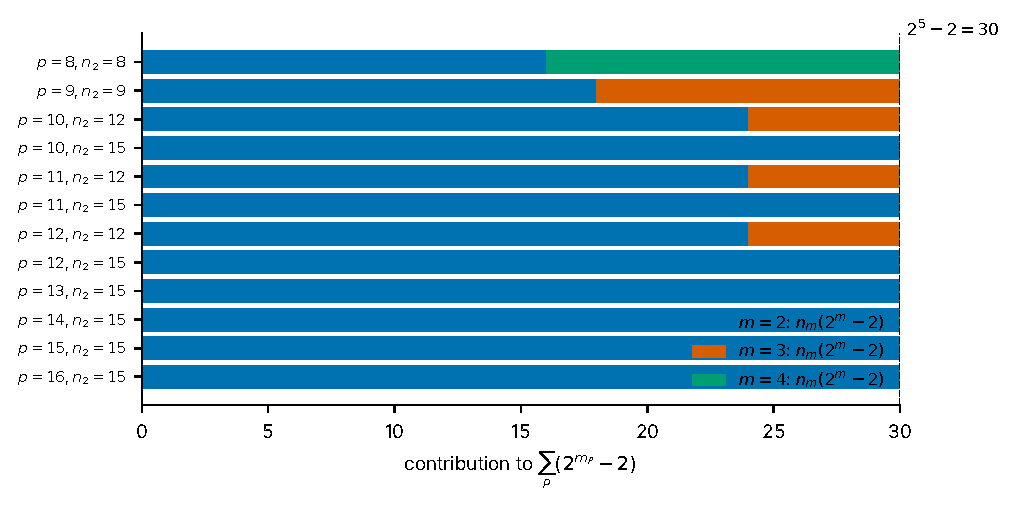
\includegraphics[width=0.95\textwidth]{figures/fig10_counting_identity.pdf}
\caption{The counting identity for the twelve minimal reduced classes with $k=5$: stacked contributions $n_m(2^m-2)$ to the total $2^k-2=30$. \figdesc{exact from the classification of Section~\ref{sec:classify}.}}\label{fig:counting}
\end{figure}

%% -------------------------------------------------------------------
\section{The second-moment (Parseval) identity}\label{sec:parseval}

For a word $w$ write $|w|=\wt(w)$.

\begin{lemma}[Second moment of the weight]\label{lem:moment}
Let $C$ be a reduced code of nullity $k$ and length $p$ (no dead coordinates, no two series-equivalent coordinates). Then
\[
\sum_{w\in C}|w|^2=2^{k-2}\,p\,(p+1).
\]
\end{lemma}

\begin{proof}
$|w|^2=\sum_{i,j}w_iw_j$. For each coordinate $i$, $\#\{w: w_i=1\}=2^{k-1}$ because the $i$th coordinate functional is nonzero on $C$. For $i\ne j$ the pair of functionals $(w\mapsto w_i,\,w\mapsto w_j)$ on $C$ is linearly independent (the coordinates are neither dead nor series-equivalent: a relation $w_i=w_j$ for all $w$ or $w_i=0$ for all $w$ is excluded), so $\#\{w:w_i=w_j=1\}=2^{k-2}$. Therefore $\sum_w|w|^2=p\,2^{k-1}+p(p-1)2^{k-2}=2^{k-2}p(p+1)$.
\end{proof}

(In coding-theoretic language the hypothesis says the dual code has minimum distance at least $3$, i.e.\ $C$ is an orthogonal array of strength~$2$; the formula is the second moment in the MacWilliams framework \cite{MacWilliamsSloane1977}.)

\begin{lemma}[Block expansion]\label{lem:block}
Let $P$ be a partition of $[p]$ into blocks of sizes $b_1,\dots,b_m$ and put $S_P=\sum_jb_j^2$. Then
\[
\sum_{w\in V_P}|w|^2=2^{m-2}\bigl(S_P+p^2\bigr).
\]
\end{lemma}

\begin{proof}
A word of $V_P$ is the union of the blocks indexed by $J\subseteq[m]$, with weight $\sum_{j\in J}b_j$. Summing over all $J$: each $b_j^2$ appears in $2^{m-1}$ subsets, each cross term $b_jb_l$ ($j\ne l$, counted twice in the square) in $2^{m-2}$, so $\sum_J(\sum_{j\in J}b_j)^2=2^{m-1}S_P+2^{m-2}(p^2-S_P)=2^{m-2}(S_P+p^2)$.
\end{proof}

\begin{theorem}[Parseval identity; \gid{G11-L5b}]\label{thm:parseval}
For a minimal non-embedded box (reduced, length $p$, nullity $k$),
\[
\sum_{P\in\Part}\bigl(2^{m_P}S_P-2p^2\bigr)=p\,(2^k-2p),
\]
where $S_P=\sum_{B\in P}|B|^2$. For a partition $P=\{B_1,B_2\}$ into two blocks the summand is $2(|B_1|-|B_2|)^2\ge0$.
\end{theorem}

\begin{proof}
Partition $C=\{0\}\sqcup\{\one\}\sqcup\bigsqcup_P(V_P\setminus\{0,\one\})$ (Theorem~\ref{thm:vsp}). The word $0$ has weight $0$ and $\one$ has weight $p$. By Lemmas~\ref{lem:moment} and~\ref{lem:block},
\[
2^{k-2}p(p+1)=p^2+\sum_P\Bigl[2^{m_P-2}(S_P+p^2)-p^2\Bigr].
\]
Multiply by $4$ and use $\sum_P 2^{m_P}=2^k-2+2\beta$ (Theorem~\ref{thm:counting}, with $\beta=|\Part|$):
\[
2^kp(p+1)=4p^2+\sum_P2^{m_P}S_P+p^2(2^k-2+2\beta)-4\beta p^2,
\]
that is, $\sum_P2^{m_P}S_P=2^kp(p+1)-4p^2-p^2(2^k-2)+2\beta p^2=2^kp-2p^2+2\beta p^2$. Subtracting $2\beta p^2$ gives $\sum_P(2^{m_P}S_P-2p^2)=2^kp-2p^2=p(2^k-2p)$. For $m=2$, $4(b_1^2+b_2^2)-2(b_1+b_2)^2=2(b_1-b_2)^2$.
\end{proof}

\src{\gid{G11-L5b}, GEO-I v011 \texttt{MATHEMATICS.md} \S1.4 (\PROVED). Re-derived here from Lemmas~\ref{lem:moment}--\ref{lem:block}; the identity was verified exactly for all $231$ classified classes with $k\le6$ (Appendix~\ref{app:repro}).}

\begin{example}[Checks]\label{ex:parseval}
$E_4$: $p=4$, $k=3$, three partitions with blocks $(2,2)$, so $S_P=8$ and each summand is $4\cdot8-32=0$; the right side is $4\,(8-8)=0$. For the $k=4$, $p=6$ box: the three-block partition has $S=12$ and summand $8\cdot12-72=24$, the right side is $6\,(16-12)=24$, so the four two-block summands $2(b_1-b_2)^2$ sum to $0$ and each two-block partition has two blocks of size~$3$. $\AG(k-1,2)$: all $2^{k-1}-1$ partitions have blocks of size $p/2$, every summand vanishes, and the right side $p(2^k-2p)=0$ because $p=2^{k-1}$.
\end{example}

\begin{remark}[Fourier-analytic reading]\label{rem:fourier}
The weight enumerator of $C$ is the Fourier transform (over the group $\F_2^k$ of functionals) of the indicator of the point set $X$, and Lemma~\ref{lem:moment} is its second moment \cite{Terras1999,ODonnell2014}. The theorem says that this second moment is also the sum of the second moments of the pieces $V_P$ of the vector-space partition, each of which is computable from the block sizes alone. This is what makes the partition data so rigid.
\end{remark}

%% -------------------------------------------------------------------
\section{Quantitative inequalities}\label{sec:ineq}

Put, for $P\in\Part$ with $m=m_P$ blocks,
\[
t_P=2^{m}S_P-2p^2-p\,(2^{m}-2).
\]
Subtracting $p$ times the counting identity from the Parseval identity gives
\begin{equation}\label{eq:tsum}
\sum_{P\in\Part}t_P=p(2^k-2p)-p(2^k-2)=-2p(p-1).
\end{equation}

\begin{lemma}[Cauchy--Schwarz]\label{lem:CS}
$S_P\ge p^2/m_P$, with equality iff all blocks of $P$ have the same size $p/m_P$.
\end{lemma}

\begin{lemma}[Block bound]\label{lem:mbound}
$2\le m_P\le p/2$ for every $P\in\Part$.
\end{lemma}

\begin{proof}
Every block has size $\ge2$ (Corollary~\ref{cor:minprops}) and the sizes add to $p$.
\end{proof}

\begin{lemma}[Two-block terms]\label{lem:t2}
If $m_P=2$ then $t_P=2(|B_1|-|B_2|)^2-2p\ge-2p$, with equality iff $|B_1|=|B_2|$.
\end{lemma}

\begin{lemma}[Threshold inequality]\label{lem:threshold}
For integers $p\ge9$ and $3\le m\le p/2$,
\[
p\Bigl(\frac{2^m}{m}-2\Bigr)\ \ge\ 2^m-2,
\]
with equality if and only if $(p,m)=(9,3)$. For $p\in\{6,7,8\}$ the inequality fails for $m=3$, and it holds strictly for $m=4$, $p=8$.
\end{lemma}

\begin{proof}
Since $2^m/m-2>0$ for $m\ge3$ the inequality is equivalent to $p\ge f(m):=\dfrac{m(2^m-2)}{2^m-2m}$ (the denominator is positive for $m\ge3$). We compute $f(3)=\frac{3\cdot6}{2}=9$, $f(4)=\frac{4\cdot14}{8}=7$, $f(5)=\frac{5\cdot30}{22}=\frac{75}{11}<7$. For $m=3$ the inequality $p\ge9$ holds with equality iff $p=9$. For $m=4$ we have $p\ge8>7$ since $m\le p/2$ gives $p\ge8$. For $m\ge5$ write $f(m)=m+\dfrac{m(2m-2)}{2^m-2m}$; then $f(m)<2m$ is equivalent to $m(2m-2)<m(2^m-2m)$, i.e.\ $2^m>4m-2$, which holds for $m\ge4$ ($16>14$) and propagates by $2^{m+1}=2\cdot2^m>8m-4\ge4(m+1)-2$ for $m\ge1$. Since $p\ge2m>f(m)$ the inequality is strict. For $p\in\{6,7,8\}$ and $m=3$: $p<9=f(3)$, so the inequality fails.
\end{proof}

\begin{table}[ht]
\centering\small
\begin{tabular}{@{}rrrrr@{}}
\toprule
$m$ & $f(m)$ & $\lceil f(m)\rceil$ & $2m$ & range of $p$ where $p\ge f(m)$ and $p\ge2m$ \\
\midrule
$3$ & $9$ & $9$ & $6$ & $p\ge9$\\
$4$ & $7$ & $7$ & $8$ & $p\ge8$\\
$5$ & $75/11\approx6.82$ & $7$ & $10$ & $p\ge10$\\
$6$ & $6\cdot62/52\approx7.15$ & $8$ & $12$ & $p\ge12$\\
$7$ & $7\cdot126/114\approx7.74$ & $8$ & $14$ & $p\ge14$\\
$8$ & $8\cdot254/240\approx8.47$ & $9$ & $16$ & $p\ge16$\\
\bottomrule
\end{tabular}
\caption{The threshold function $f(m)=m(2^m-2)/(2^m-2m)$. For every $m\ge4$ one has $f(m)<2m$, so the constraint $m\le p/2$ already forces $p>f(m)$. Only $m=3$ imposes a nontrivial lower bound, $p\ge9$.}\label{tab:threshold}
\end{table}

\begin{corollary}[Sign of the higher terms]\label{cor:tpos}
If $p\ge9$ then $t_P\ge0$ for every $P\in\Part$ with $m_P\ge3$, and $t_P>0$ unless $(p,m_P)=(9,3)$ and all three blocks have size $3$.
\end{corollary}

\begin{proof}
By Lemma~\ref{lem:CS}, $t_P\ge p\bigl[p(2^m/m-2)-(2^m-2)\bigr]$ with $m=m_P\le p/2$; apply Lemma~\ref{lem:threshold}. Equality forces $(p,m)=(9,3)$ and equality in Cauchy--Schwarz.
\end{proof}

\begin{remark}[The exceptional finite range]\label{rem:exceptional}
For $p\le8$ the bound of Corollary~\ref{cor:tpos} fails only for $m=3$ (which requires $p\ge6$), and only for $p=6,7,8$. There the Cauchy--Schwarz bound gives $t_P\ge p\bigl[\tfrac23p-6\bigr]$, i.e.\ $-12$, $-\tfrac{28}{3}$ and $-\tfrac{16}{3}$ for $p=6,7,8$ (Appendix~\ref{app:I}). With such negative terms permitted, the identities and inequalities alone do not exclude a profile with at most one two-block partition: the supplementary scan \gid{G11-V1} of the source reports, for $k=5$, one numerically feasible profile with $p=6$ which no code realizes (our enumeration in Table~\ref{tab:smallp} finds no minimal box at $(k,p)=(5,6)$). The cases $p\le8$ are therefore treated by exhaustive enumeration (Section~\ref{sec:W2}).
\end{remark}

%% -------------------------------------------------------------------
\section{At least \texorpdfstring{$p-1$}{p-1} two-block partitions}\label{sec:n2}

\begin{theorem}[$n_2\ge p-1$; \gid{G11-L6}]\label{thm:L6}
Let $C$ be a minimal non-embedded box (reduced, length $p\ge9$, nullity $k$). Then
\[
n_2\ \ge\ p-1 .
\]
If $p\ge10$ then equality holds if and only if $X=\AG(k-1,2)$ (so $p=2^{k-1}$ and $C=\mathrm{RM}(1,k-1)$). If $p=9$ equality is impossible, so $n_2\ge9$.
\end{theorem}

\begin{proof}
By~\eqref{eq:tsum}, $-2p(p-1)=\sum_Pt_P$. Split into two-block and higher partitions. Lemma~\ref{lem:t2} gives $\sum_{m_P=2}t_P\ge-2p\,n_2$ and Corollary~\ref{cor:tpos} gives $\sum_{m_P\ge3}t_P\ge0$. Hence $-2p(p-1)\ge-2pn_2$, i.e.\ $n_2\ge p-1$.

\emph{Equality.} If $n_2=p-1$ all inequalities are tight: every two-block partition is balanced (blocks of size $p/2$) and $\sum_{m_P\ge3}t_P=0$. For $p\ge10$ Corollary~\ref{cor:tpos} gives $t_P>0$ for every $m_P\ge3$, so there is no partition with $m_P\ge3$. Then the counting identity reads $2n_2=2^k-2$, so $p-1=n_2=2^{k-1}-1$ and $p=2^{k-1}=|H|$: $X=H=\AG(k-1,2)$. Conversely $X=\AG(k-1,2)$ has $n_2=p-1$ by Proposition~\ref{prop:RM}. For $p=9$, equality would force every $m_P\ge3$ partition to have $m_P=3$ with blocks $3,3,3$ (the exceptional case of Corollary~\ref{cor:tpos}) and so $2\cdot8+6n_3=2^k-2$, i.e.\ $2^k=18+6n_3$ is divisible by $3$, which is absurd.
\end{proof}

\src{\gid{G11-L6}, GEO-I v011 \texttt{MATHEMATICS.md} \S1.5 (\PROVED+\CHECKED); sharpness \gid{G11-K1} (\CHECKED in the source). The characterisation of the equality case for $p\ge10$ and the impossibility for $p=9$ are made explicit here (new here). The bound was confirmed on all $231$ classified classes and on $19\,373$ labelled minimal subsets for $k=5$ (min $n_2=8$).}

\begin{proposition}[The Reed--Muller family]\label{prop:RM}
For $k\ge3$ let $X=\AG(k-1,2)$ (all $p=2^{k-1}$ points of $H$) and $C=\mathrm{RM}(1,k-1)$. Then the circuits are the $2^k-2$ words of weight $p/2$; the partitions of $\one$ are the $2^{k-1}-1$ pairs $\{w,\one\oplus w\}$; $n_2=p-1$; $C$ is minimal non-embedded; $\rmin=3$.
\end{proposition}

\begin{proof}
The words are the affine functions on $\F_2^{k-1}$: $0$, $\one$ and $2^k-2$ words of weight $p/2$. Distinct nonzero words of equal weight are not nested, and every word other than $0,\one$ is nonconstant and has weight $p/2$, so the circuits are exactly the $2^k-2$ words of weight $p/2$ (the word $\one$ contains each, so is not a circuit). Two disjoint circuits have total weight $p$, hence are complementary: the partitions of $\one$ are the pairs $\{w,\one\oplus w\}$, of which there are $(2^k-2)/2$. For $k\ge3$ this is $\ge3$, so $C$ is non-embedded by Theorem~\ref{thm:E1}. Shortening at a coordinate $i$: the circuits avoiding $i$ are the $w$ with $w_i=0$; two disjoint ones are complementary, so one of them contains $i$: contradiction. Hence no set is partitioned into two or more circuits in $C_{(i)}$, every set has at most one partition, and $C_{(i)}$ is embedded. Rank three follows from Theorem~\ref{thm:L5}.
\end{proof}

\src{\gid{G8-T3c}, GEO-I v008 \texttt{MINIMAL\_RANK.md} (\PROVED, \CHECKED for $k=3,4,5$); re-proved above by a direct argument.}

\begin{figure}[ht]
\centering
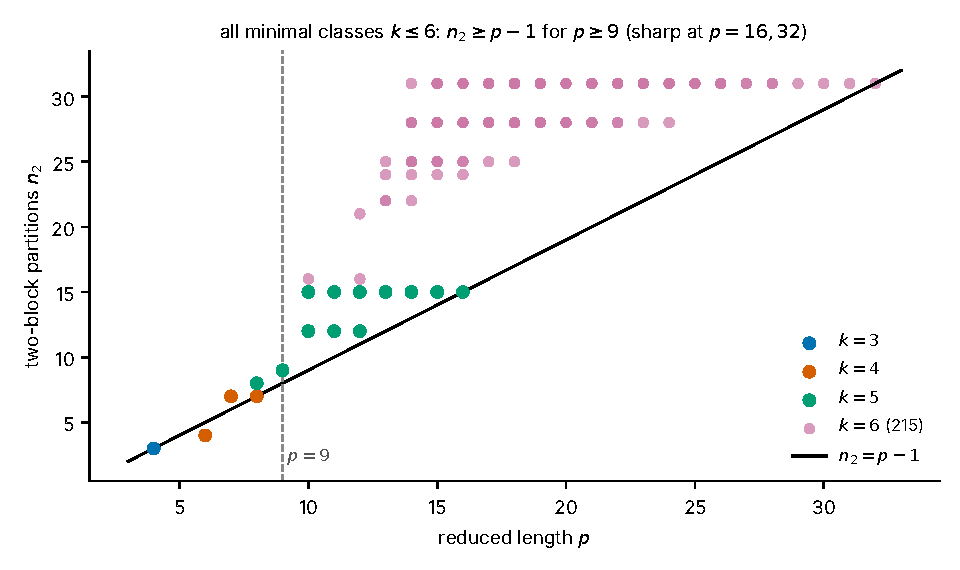
\includegraphics[width=0.95\textwidth]{figures/fig11_n2_bound.pdf}
\caption{The number $n_2$ of two-block partitions against the reduced length $p$ for all minimal classes with $k=3,\dots,6$ ($231$ classes), with the line $n_2=p-1$ and the threshold $p=9$. Points on the line are the Reed--Muller supports $p=4,8,16,32$. \figdesc{exact data; for $k=6$ from the source-reported list of $215$ representatives recomputed with the independent engine.}}\label{fig:n2}
\end{figure}

%% -------------------------------------------------------------------
\section{W2 universality}\label{sec:W2}

The inequality of Section~\ref{sec:n2} settles $p\ge9$. For $p\le8$ we use a normal form that reduces the problem to a very small enumeration.

\begin{lemma}[Simplex normal form]\label{lem:simplex}
Let $X\subseteq H\cong\AG(k-1,2)$ be a spanning subset with $|X|=p$. Then $X$ is $\AGL(k-1,2)$-equivalent to a set
\[
\{e_1,\dots,e_k\}\cup R,\qquad R\subseteq O_k,\ |R|=p-k,
\]
where, in suitable coordinates, $H$ is the set of odd-weight vectors of $\F_2^k$ and $O_k$ is the set of odd-weight vectors of weight $\ge3$.
\end{lemma}

\begin{proof}
$X$ spans $\F_2^k$, so it contains a basis $b_1,\dots,b_k$. Since $f_0(b_i)=1$ for all $i$, in the basis $(b_i)$ the functional $f_0$ is $(1,\dots,1)$, so $H$ is the set of odd-weight vectors and $b_i=e_i$. The change of basis fixes $f_0$, hence induces an element of $\AGL(k-1,2)$ (Section~\ref{sec:affine}). The remaining points of $X$ are odd-weight vectors different from $e_i$, i.e.\ of weight $\ge3$.
\end{proof}

\begin{proposition}[Finite check for $p\le8$]\label{prop:small}
For every pair $(k,p)$ with $3\le k<p\le8$ let $\mathcal N_{k,p}$ be the set of subsets $R\subseteq O_k$ with $|R|=p-k$ (so $\binom{|O_k|}{p-k}$ candidates). For each candidate the reduced box $\{e_1,\dots,e_k\}\cup R$ was tested for non-embeddedness (Theorem~\ref{thm:E1}, direct enumeration of circuit partitions), minimality (non-embeddedness of every shortening), and $n_2$ (the number of partitions of $\one$ into two circuits). The results are in Table~\ref{tab:smallp}: minimal boxes occur only for $(k,p)\in\{(3,4),(4,6),(4,7),(4,8),(5,8)\}$ and they have $n_2\ge3$.
\end{proposition}

\begin{table}[ht]
\centering\small
\begin{tabular}{@{}rrrrrr@{}}
\toprule
$p$ & $k$ & candidates & non-embedded & minimal & $\min n_2$ over minimal\\
\midrule
\smallptablebody
\bottomrule
\end{tabular}
\caption{The finite enumeration for $p\le8$ (Proposition~\ref{prop:small}). ``Candidates'' counts the sets $R\subseteq O_k$ of size $p-k$. All candidates are non-embedded. Minimal boxes with $p\le8$ exist only for the pairs $(k,p)=(3,4),(4,6),(4,7),(4,8),(5,8)$; for $(k,p)=(5,8)$ ten of the $165$ candidates are minimal.}\label{tab:smallp}
\end{table}

\src{New here as a self-contained route (Appendix~\ref{app:K}); \texttt{scripts/small\_p.py}, own code. The source proves W2 for $p\le8$ via the classification through nullity $6$ (\gid{G11-T3}, \texttt{MATHEMATICS.md} \S1.7) and the exclusion of $(k,p)=(7,8)$ (\gid{G11-L6b}). Both routes agree. Status of Proposition~\ref{prop:small}: \PROVED+\CHECKED (exhaustive, complete, $655$ candidates in total; no hand proof).}

\begin{figure}[ht]
\centering
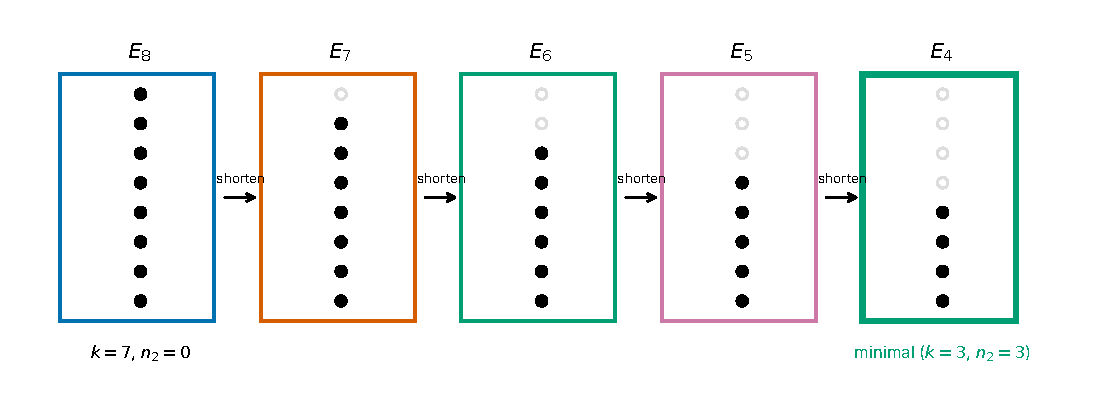
\includegraphics[width=0.95\textwidth]{figures/fig13_E8_nonminimal.pdf}
\caption{The case $(k,p)=(7,8)$: $C=E_8$ with its $28$ weight-two circuits and $105$ perfect matchings of the coordinates, but no partition of $\one$ into two circuits. $E_8$ is not minimal because shortening gives $E_7$, then $E_6,E_5,E_4$, which is the minimal sub-box on four coordinates. \figdesc{schematic chain of shortenings; the sub-box $E_4$ sits on any four of the eight coordinates.}}\label{fig:E8}
\end{figure}

\begin{theorem}[W2 universality; \gid{G11-T3}]\label{thm:W2}
Every minimal non-embedded box satisfies W2: the all-ones word has at least two partitions into exactly two circuits, i.e.\ $n_2\ge2$. More precisely, if $p\ge9$ then $n_2\ge p-1\ge8$, and if $p\le8$ then $n_2\ge3$.
\end{theorem}

\begin{proof}
If $p\ge9$, Theorem~\ref{thm:L6}. If $p\le8$, the reduced code is a spanning subset of $\AG(k-1,2)$ with $k+1\le p\le8$ points (Theorem~\ref{thm:affine}), hence equivalent to one of the candidates of Proposition~\ref{prop:small} by Lemma~\ref{lem:simplex}; by Table~\ref{tab:smallp} every minimal one has $n_2\ge3$. The cases with $p=k+1$ are consistent with this: they are the even-weight codes $E_p$, minimal only for $p=4$ (Proposition~\ref{prop:Emin}); in particular the case $(k,p)=(7,8)$ ($C=E_8$, with $28$ circuits of weight two, $105$ perfect matchings and $n_2=0$) is not minimal.
\end{proof}

\src{\gid{G11-T3} (= \gid{G10-C1} = \gid{G11-C2}), GEO-I v011 \texttt{MATHEMATICS.md} \S1.7 (\PROVED+\CHECKED). The part for $p\ge9$ is proved in the text without any enumeration. The part for $p\le8$ rests on the exhaustive enumeration above (and, in the source, on the classification for $k\le6$ and \gid{G11-L6b}).}

%% -------------------------------------------------------------------
\section{The main theorem: universal rank three}\label{sec:main}

\begin{theorem}[Universal minimum witness rank; \gid{G11-T4}]\label{thm:rank3}
For every non-embedded box $C$ of the frozen binary $0/1$ Graver-cell model, of arbitrary length $n$, nullity $k$ and parity matrix (zero columns included),
\[
\rmin(C)=3 .
\]
The value $3$ is attained by a collision of two cells of dimension~$2$ obtained from two two-circuit partitions of $\one$ in a minimal sub-box.
\end{theorem}

\begin{proof}
Theorem~\ref{thm:W2} shows that every minimal non-embedded box satisfies W2. Theorem~\ref{thm:C1p} (descent to a minimal sub-box, Theorem~\ref{thm:L5} for the upper bound, Lemma~\ref{lem:LOW} for the lower bound) yields $\rmin(C)=3$.
\end{proof}

\src{\gid{G11-T4}, GEO-I v011 \texttt{RANK\_UNIVERSAL.md} (\PROVED). All steps are proved in this paper except the finite enumeration of Proposition~\ref{prop:small}.}

\begin{corollary}[No minimal box of rank four]\label{cor:no4}
No minimal non-embedded box has $\rmin\ge4$. Consequently the conjecture \gid{G10-C2} (``a minimal box with $\rmin=4$ exists'') is false in the frozen model, and the statement ``$\rmin\ge4$ implies nullity $\ge7$'' (\gid{G10-T4}) is vacuous.
\end{corollary}

\src{\gid{G11-C3}: status \textsc{false} for \gid{G10-C2}, GEO-I v011 \texttt{RANK\_UNIVERSAL.md}.}

\begin{remark}[What the theorem does not say]\label{rem:notalg}
(i)~Individual collisions can have large rank (Remark~\ref{rem:individual}). (ii)~The theorem is about the \emph{existence} of a rank-three collision in every non-embedded box; it gives no bound on how hard it is to \emph{find} one. (iii)~The theorem is for the frozen binary model only. (iv)~The proof of W2 for $p\le8$ is by a complete but computer-executed enumeration; the proof for $p\ge9$ is a hand proof.
\end{remark}

\begin{figure}[ht]
\centering
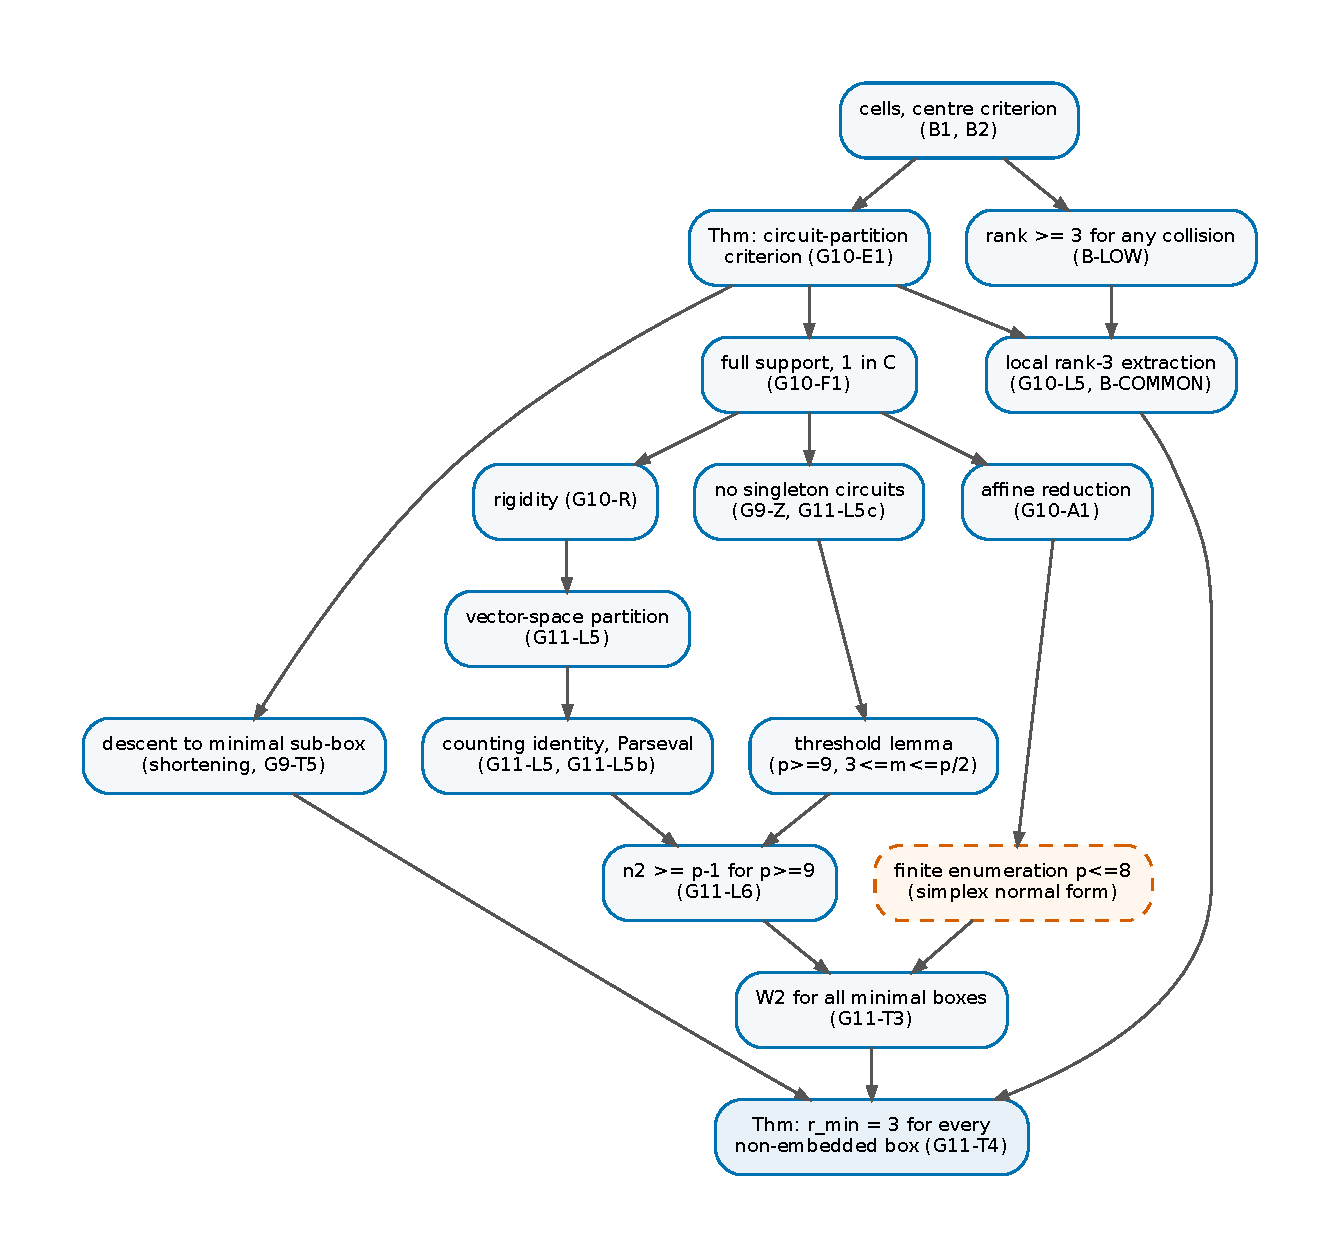
\includegraphics[width=0.95\textwidth]{figures/fig14_dependencies.pdf}
\caption{Dependency diagram of the proof. Arrows point from a result to the results that use it. Dashed boxes mark the finite enumeration ($p\le8$) and the supplementary source-reported material (nullity-$6$ classification), which is not used in the proof of the main theorem. \figdesc{generated by \texttt{scripts/figs.py}.}}\label{fig:deps}
\end{figure}
